\documentclass[conference]{IEEEtran}

\usepackage{amsmath,amssymb,amsfonts}
\usepackage{graphicx}
\usepackage{textcomp}
\usepackage{xcolor}
\usepackage[hidelinks]{hyperref}
\usepackage{algorithm}
\usepackage{algcompatible}
\usepackage{algpseudocode}
\usepackage[noadjust]{cite}
\usepackage{listings}
\lstdefinestyle{mystyle}{
    basicstyle=\ttfamily\footnotesize,
    breakatwhitespace=false,         
    breaklines=true,                 
    captionpos=b,                    
    keepspaces=true,                 
}
\lstset{style=mystyle}

\begin{document}

\title{
	PChord: Towards A Error-Free Distributed Hash Table using P
}

\author{
	\IEEEauthorblockN{Shinwoo Kim}
	\IEEEauthorblockA{
		\textit{Department of Computer Science} \\
		\textit{University of Pittsburgh} \\
		Pittsburgh, USA \\
		\href{mailto:shinwookim@pitt.edu}{shinwookim@pitt.edu}
		} \and
	\IEEEauthorblockN{Derrick Hicks}
	\IEEEauthorblockA{
		\textit{Department of Computer Science} \\
		\textit{University of Pittsburgh} \\
		Pittsburgh, USA \\
		\href{mailto:ddh32@pitt.edu}{ddh32@pitt.edu}
	}
}

\maketitle

\begin{abstract}
	Building distributed systems is challenging, and ensuring their correctness even more so. To address this difficulty, most systems rely on a formal-methods approach to ensure that they are \textit{correct}, and software testing to ensure that they are free of bugs. In this paper, we examine P, an asynchronous event-driven programming language that combines model-checking and programming into one activity for the developer. With P, we develop the Chord distributed hash table protocol, and analyze the broader system-building process facilitated by P.
\end{abstract}

\section{Introduction}
Peer-to-peer (P2P) computing is a decentralized network architecture where participants, known as peers, share resources directly with each other without relying on a central server. In these systems, each peer acts as both a client and a server, enabling a more distributed and autonomous approach to communication and resource sharing. However, because there is no singular coordinator, a fundamental problem in P2P computing is how best to locate a particular resource.

One solution to this \textit{look-up problem} is the Chord protocol, which provides a way of storing and efficiently retrieving key-node mappings in a decentralized way~\cite{stoica_chord_2001,stoica_chord_2003,liben-nowell_analysis_2002}. In essence, Chord takes the idea of a hash table and expands it to a distributed setting. That is, each resource is given a key $k_i$ which Chord can use to efficiently determine which node the resource associated with it is being stored. The Chord protocol is described with more detail in \autoref{sec:chord}.

Unfortunately, correctly implementing the Chord protocol is not a trivial task. More generally, distributed systems are notorious for being hard to get right, and decentralized ones are even harder to work with. One must be able to effectively reason about concurrent execution on multiple machines and have a deep understanding of the underlying protocols and assumption that allows for effective and error-free communication across a network; at the same time, they must ensure no subtle logical and programmatic bugs are introduced into the system. Indeed, recent work has shown that there are many bugs both in the Chord protocol and many of its implementations that threaten Chord's correctness guarantees~\cite{zave_reasoning_2017}.

To mitigate this issue, system builders typically take a two-phase approach~\cite{newcombe_how_2015}. At the protocol level, protocol designers write high-level specifications (using specialized languages like TLA+ or Alloy) that mathematically captures the semantics and properties of the system; these specifications are then formally validated using proof-based verification, or model-checking where user-specified invariants are shown to hold for all possible states~\cite{jackson_alloy_2002,lamport_tla_1994}.

At the implementation-level, developers carefully read the high-level specification and translate it into an executable program using a programming language like Python, Go, or Java. Special care needs to be taken to ensure that the implementation accurately conforms to the specification, but once an implementation is ready, it also undergoes extensive testing, such as unit and integration testing. 

g
The P programming language is an attempt to make it easier for developers writing \textit{provably correct} distributed systems. P does this by ``unifying and programming into one activity for the programmer''~\cite{desai_p_2013}. Specifically, P allows the programmer to specify the system as a set of event-driven state machines and provides extensive tooling to test the system using model checking techniques. We briefly discuss the P language below in \autoref{sec:P}, but a more thorough examination can be found in~\cite{desai_p_2013}.

In this paper, we make the following contributions:
\begin{enumerate}
	\item An implementation of the Chord protocol using P which can guarantee correctness via model-checking.
	\item An examination of the system design process in P and an analysis of the limitations of P.
\end{enumerate}
The source code for PChord can be found at \url{https://github.com/shinwookim/PChord}.

\begin{figure}[ht!]
	\centering
	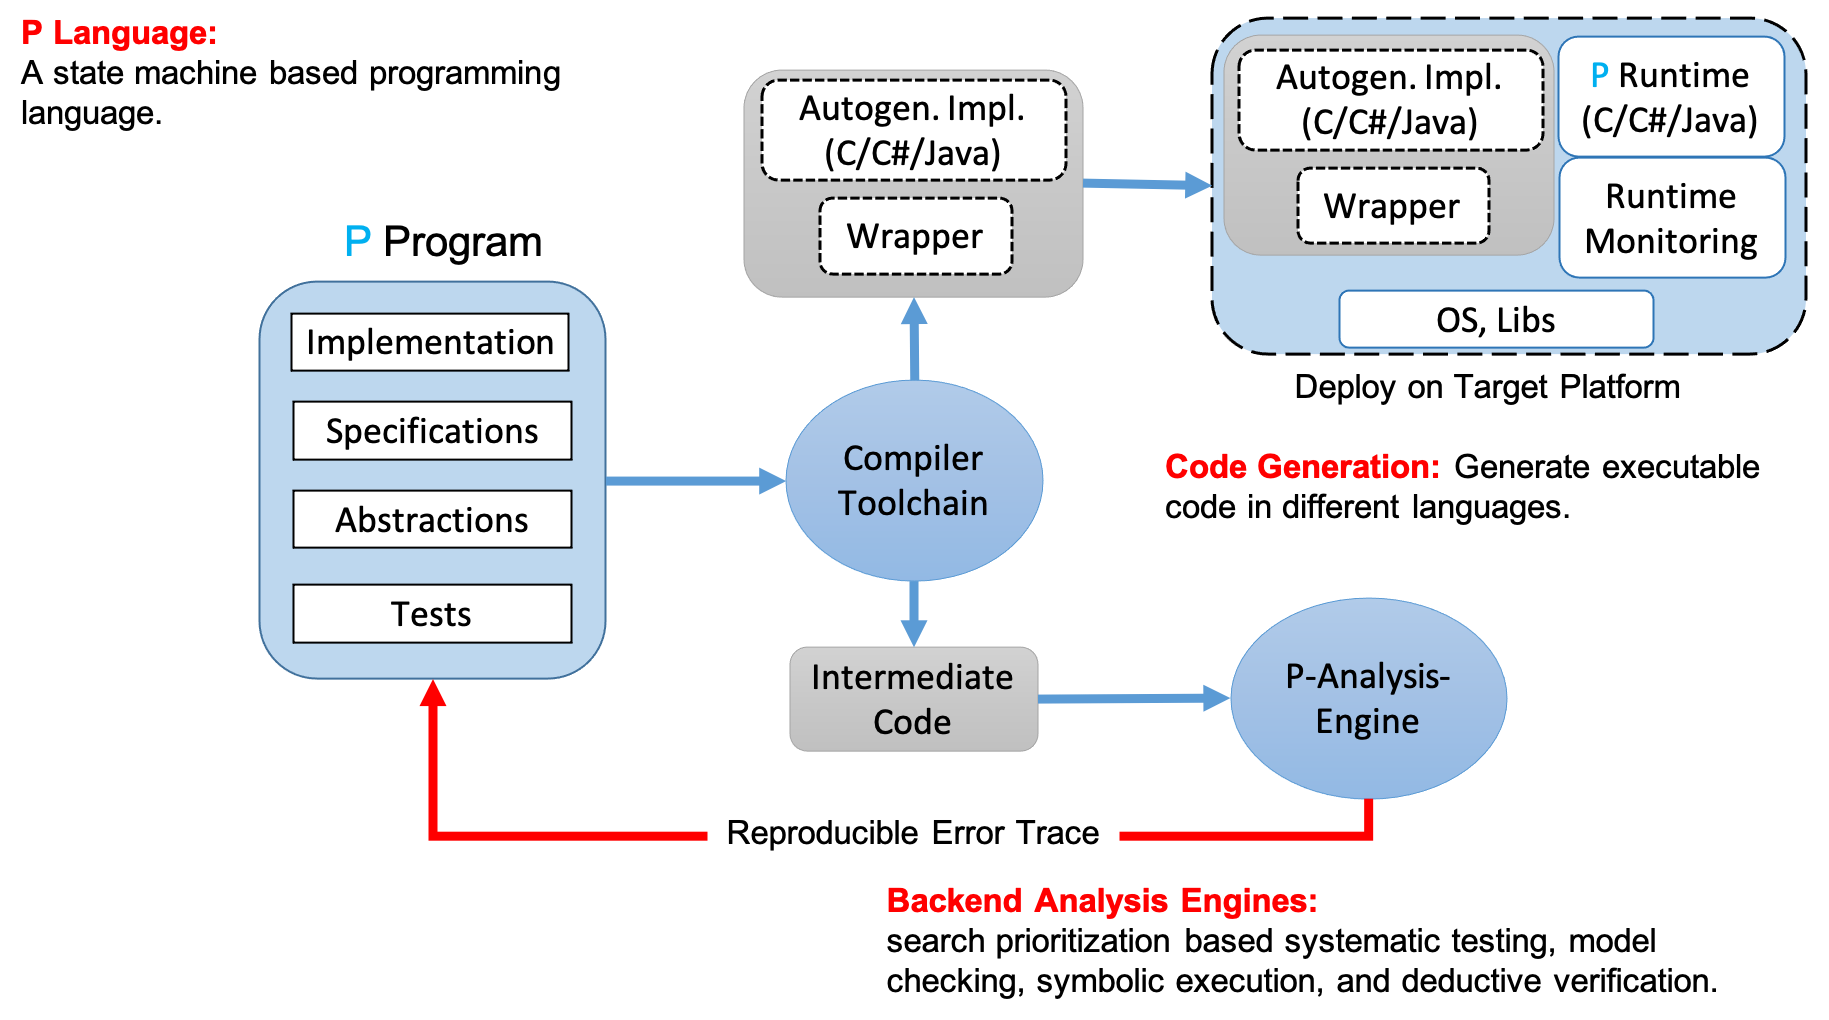
\includegraphics[width=\linewidth]{p-toolchain.png}
	\caption{P Programming Language Framework \& Architecture. Figure from \cite{p_developers_formal_2023}.}
	\label{fig:p-framework}
\end{figure}

\subsection{P Language}\label{sec:P}
The P programming language is a domain-specific language designed for writing asynchronous, event-driven code. P enables programmers to specify a system as a collection of interacting state machines that communicate with each other using events. Importantly, the semantics of these state machines are both interpretable by P's model checker and compiler, thereby unifying the modeling and implementation tasks of building systems into a single framework~\cite{desai_compositinal_2018}.

The P framework consists mainly of three parts, as shown in \autoref{fig:p-framework}. P provides a high-level \textit{state machine-based programming language} that can be used to formally model and specify (distributed) systems. This way of capturing systems and protocols as state machine is a common way of reasoning for many programmers, so P does not cause an undue hardship for the programmer~\cite{deligiannis_programming_2015}. Importantly, P's syntax tries to balance the \textit{formalism} of a mathematical modelling language and the \textit{expressiveness} of a programming language to allow developers to both easily create models that conform to the actual system and maintain them. An example of P's syntax can be seen in \autoref{fig:p-syntax}.

\begin{figure}[h]
	\centering
	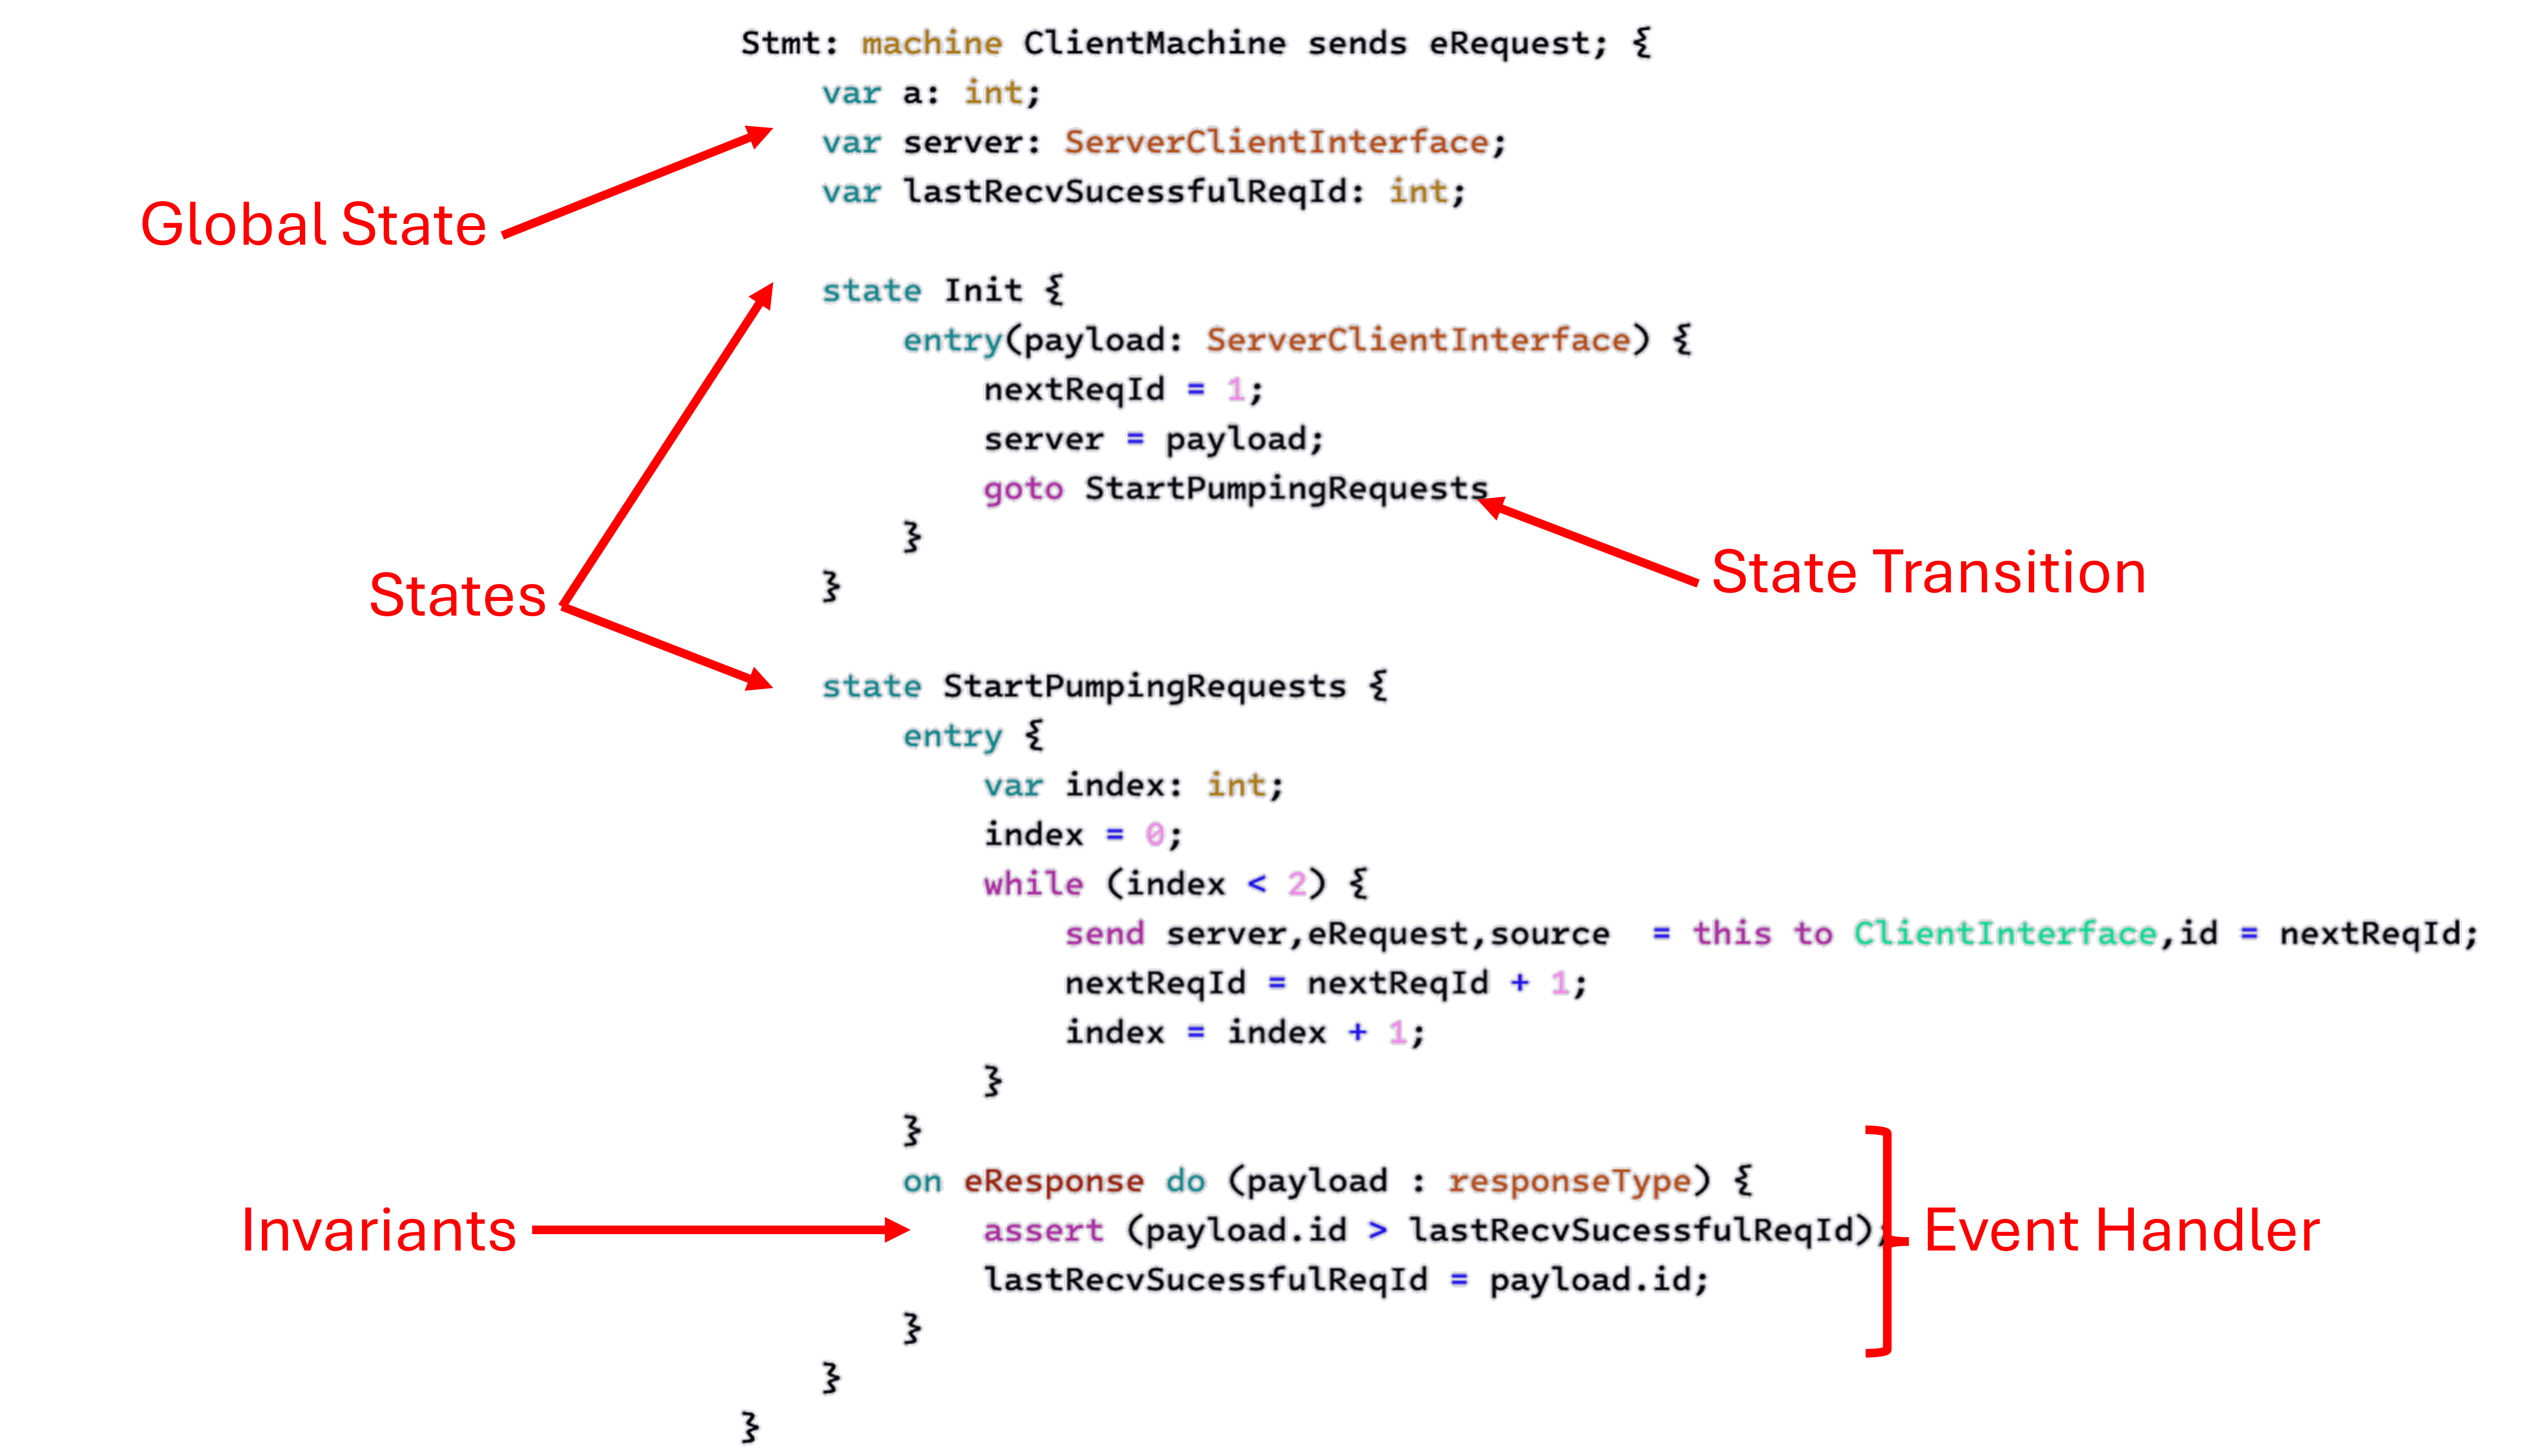
\includegraphics[width=\linewidth]{p-annotated.png}
	\caption{A (annotated) sample program written in the P language.}
	\label{fig:p-syntax}
\end{figure}

Once a P program has been specified, it is fed to the compiler tool chain, which can either generate executable or intermediate code. The executable code takes the form of C/C\# code, which allows the system to be easily deployed or integrated with other systems and code. The intermediate code is used by P's backend analysis engine to perform model-checking; the P model checker uses the intermediate representation to perform a systematic search of the possible state space to uncover bugs. Importantly, both the executable code and the model-checking code is generated from the same source.

P was originally developed by Microsoft, but it has since been open-sourced. Most notably, P was recently used to implement and verify the core USB driver stack for Microsoft Windows 8. A more in-depth discussion of the internals of P can be found on the language's website: \url{https://p-org.github.io/P/} \cite{p_developers_formal_2023}.



\subsection{Chord Protocol}\label{sec:chord}
The Chord protocol is based on \textit{consistent hashing} which is a way of assigning keys to nodes in a way that minimizes key migration, as much as possible, when a new node joins or an old node leaves~\cite{karger_consistent_1997}. Importantly, Chord, at its core, is designed to support the following primitive operation: 
\begin{quote}
	\texttt{Lookup($k_i)$}: given key $k_i$, determine the node that is responsible for storing it.
\end{quote}
High-level software, such as many distributed hash table implementations, use this fundamental operation as a building block to provide a wide variety of functionalities.

Internally, Chord assigns a unique key (or identifier) to both resources and nodes; e.g., a node identifier may be generated by applying a SHA128 hash function onto that node's IP address. These identifiers are organized in a ring structure, similar to the one shown in \autoref{fig:chord}. A node then is responsible for all keys whose \textit{successor} is that node's identifier, where $$\text{sucessor}(k_i) = k_j$$ iff $k_j$ refers to a node and is the first identifier that is encountered in the ring while traversing clockwise from the position of $k_i$. For instance, in \autoref{fig:chord}, the successor of key $6$ is $0$, so the resource referenced by key $6$ is stored at node $0$. Using this definition, Chord defines a look-up algorithm, similar to the one shown in Algorithm \autoref{alg:chord-lookup}.

\begin{algorithm}[ht]
	\caption{Chord Look-up Algorithm (Simplified)}
    \label{alg:chord-lookup}
	\begin{algorithmic}
		\State {my\_id} $=$ identifier for current node 
		\Procedure{Lookup}{key $k_i$}
		\State succ $\gets$ \Call{GetSuccessor}{current node}
		\If{my\_id $<$ succ $<$ $k_i$}
		\State \Call{Lookup}{$k_i$} on node succ
		\Comment{Hop to next node}
		\Else
		\State \Return succ \Comment{Done}
		\EndIf
		\EndProcedure
	\end{algorithmic}
\end{algorithm}

Once \texttt{lookup} determines which node is responsible for storing the key $k_i$, a Chord node can use a data structured called a \textit{finger table} to find the routing information to that node. So, in \autoref{fig:chord}, performing a \texttt{Lookup(6)} operation from any node might return node 0's IP address.
\begin{figure}
	\centering
	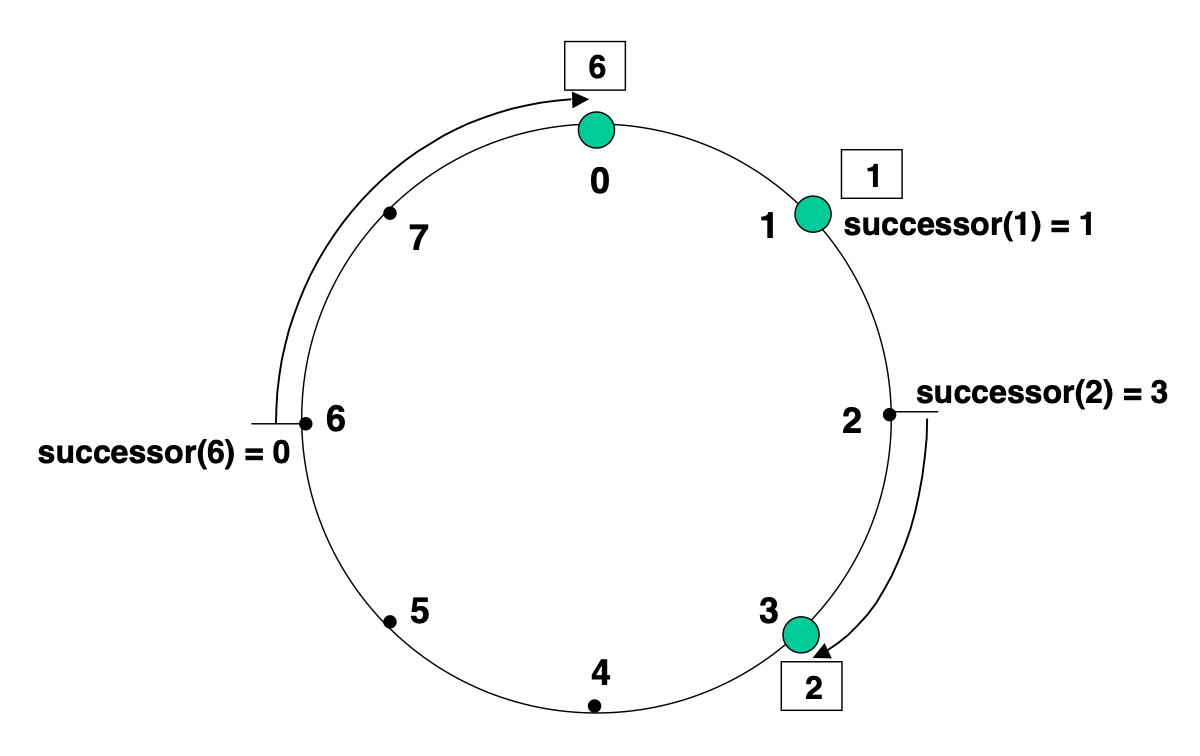
\includegraphics[width=\linewidth]{chord.png}
	\caption{
		A simple example of a Chord network consisting of three nodes with IDs $0$, $1$, and $3$. Blue dots indicate the presence of a node with that identifier.
	}
	\label{fig:chord}
\end{figure}

Besides lookup, Chord also provides a way of dealing with node joins and node exits. Essentially, when a node $k_i$ joins, certain subset of key-value pairs assigned to node \texttt{successor($k_i$)} now get reassigned to node $k_i$ such that the above property holds. Similarly, when node $k_i$ leaves, all of its key-value pairs get reassigned to node \texttt{successor($k_i$)}. There are some subtly and more detail to this process, but we omit them here for space. A fuller description of the Chord protocol can be found in \cite{stoica_chord_2001}.

\section{Approach}
In this section, we describe the design of our PChord system. In particular, we place an emphasis on the system design and validation \textit{process} when using P. For both system design and validation of correctness, we first discuss how we constructed a high-level model based on the claims in protocol description (e.g., \cite{stoica_chord_2001}). Then, we discuss the process of translating those high-level ideas into P code.

\subsection{Designing the System}
\label{sec:system-design}
As discussed in \autoref{sec:P}, P requires systems to be formulated in terms of state machines and their interactions. Some protocols and systems (e.g., many Byzantine Fault Tolerance protocols) are already synthesized this way, but others, like Chord, are not. Thus, the first task in creating a P-verified system is to create a representation of the system that is based on state-machines. Luckily, there has been a great deal of previous work that focuses on proving Chord's correctness using formal methods~\cite{zave_reasoning_2017,zave_using_2012,lund_verification_2019}. Most of these approaches use specialized modeling languages like TLA+ or Alloy, but the process of translating state machines from TLA+ or Alloy into a P-acceptable format is relatively straight forward; the difficult part is identifying what ``states'' and ``transitions'' exist in the system, not writing them in P. Hence, for PChord, we based our state-machine design based on the TLA+ model that is presented in \cite{lund_verification_2019}.

Note however that even without existing models, we believe that coming up with a state-machine based design for a protocol should not cause too much difficulty, at least for most distributed systems. Reasoning about distributed systems as state machines (sometimes called \textit{state machine replication}) is a common way of thinking for many system builders, and there exists a large corpus of work on the ``\textit{state machine approach}''~\cite{schneider_implementing_1990}.

The real challenge of writing state-machine models for P comes from the complexity of incorporating both specification and execution details into the model. Other formal methods approaches, like TLA+ and Alloy, can simplify and overlook certain details in a model that are not necessarily prudent for proving correctness; however, since P requires both execution logic and correctness specifications to be present within the model, this is not possible. For example, whereas a TLA+ model for Chord might only need to guarantee that a successor node exists, our P model must also incorporate information about how to find and contact the successor node, so that it can be used in execution. 

\subsection{PChord State-Machine Design}
In \autoref{sec:system-design}, we described how to design a state-machine based system in P. In this section, we discuss our PChord design which we created using that approach.


All systems that are formulated with state-machines as a basis must have an initial state. For Chord, the initial state is not particularly useful since a ring structure has not yet been set up. So, the first thing the system needs to do once it launches is to set up that ring structure in a process called \textit{initialization}. In our design, initialization begins with an event called `eConfig' which transfer the node from the initial state to the `WaitForRequests' state. To ensure fault-tolerance, nodes maintain a list of consecutive successors, as to allow up to $R$ node failures. This list asserts that in the case of an individual node(s) failing, the system can continue to function properly. In addition, a predecessor relationship is maintained to stabilize the network. Nodes respond to simple client key requests upon events `eAddKeyReq' and `eGetKeyReq'. If a key falls within the node's ownership, it responds accordingly; otherwise, the node forwards the client query to the appropriate successor using the `eFindSuccessorReq' event. 

To ensure the network is stable, nodes add `eStabilize' and `eFixSuccessorList' to their event buffer. When an `eStabilize' event occurs, the node queries the immediate successor to determine who their predecessor is, and verify if that predecessor is a more qualified successor (e.g., for node $5$, node $6$ is a better successor than node $7$). Once verified, the node will notify their immediate successor of their existence to maintain consistency. Upon `eFixSuccessorList', the node will query the successor to verify that it has not failed, and if it has not, to adopt its list of successors to maintain live successors. 

To simulate node failure, we utilize the P Failure Injector that arbitrarily chooses to send an `eShutdown' event to. When a node receives this event, it moves to the \textit{Unavailable} state, in which the node can either ignore a request, or respond with the `eNodeUnvailable' event (to simulate a time-out mechanism). It should be noted that a request for `eFindSuccessor' to an unavailable node will be ignored and  be lost. We rely upon the network periodic stabilization events to maintain network correctness, so that when a client "retries", it would have received a response the second time.

\subsection{Measuring Correctness}
\label{sec:measure-correctness}
To validate the correctness of a protocol and its implementation, one must first clearly define what it means for a protocol to be \textit{correct}. Previous work studying Chord have produced a list of invariants related to the Chord protocol \cite{stoica_chord_2003}, but not all of them relate to correctness. For instance, some invariants are related to probabilistic and quantitative claims regarding space-time complexity. Furthermore, some other invariants have been questioned, doubted, or refined, mainly in \cite{zave_using_2012}. Thus, after a literature review, we finalized on the following requirements (based on \cite{zave_reasoning_2017,lund_verification_2019}):
\begin{itemize}
    \item \textbf{Type Safety.} At no point should the protocol permit nodes to have successors linking to invalid destinations.
    \item \textbf{Deadlock Freedom.} There should always be at least one node so that the protocol can proceed.
    \item \textbf{Network Safety.} The protocol should not allow actions that partition the network or leave it in a state where it cannot become ideal.
    \item \textbf{Network Liveness.} After all nodes have finished joining, the protocol should eventually have arranged the network into an ideal state.
\end{itemize}
Of these, we focus on the first three, which relate to Chord's \textit{safety} properties. P's model-checker does support checking for both safety and liveness guarantees, but writing specifications and tests for safety and liveness varies somewhat. We discuss this more in \autoref{sec:towards-full-verification}.

Once we have finalized our requirements, we next need to construct appropriate specifications. These high-level specifications should be \textit{abstract} (i.e., not P code) but reveal enough so that it can eventually be refined into P code. For some requirements, it may suffice to re-write them using a more formal/precise language. For instance, to guarantee Deadlock Freedom, we may specify that there always exists a non-empty set of ring members. For others, we may need to apply knowledge about the protocol's implementation to get something that can be tested. E.g., to guarantee Type Safety, we may need to specify that all nodes are on the same ring; i.e., that only one ring exists. Listed below is a sample of the specifications we have formulated:
\begin{itemize}
    \item \textbf{(AtLeastOneRing).} There must be a ring, which means there must be a non-empty set of ring members.
    \item \textbf{(AtMostOneRing).} There must be no more than one ring, which means that from each ring member, every other ring member is reachable by following the chain of successors.
    \item \textbf{(OrderedRing).} On the unique ring, the nodes must be in identifier order.
\end{itemize}

The final step in this process is writing specifications with P. \autoref{spec-demo} shows an example of a specification that has been written in P.
\begin{lstlisting}[caption=An example specification for Chord in P,label=spec-demo]
spec AtLeastOneRing observes eSuccessorAltered, eMonitor_AtomicityInitialize, eInitalizeSuccessors
{
var successorMap: map[int, seq[tNode]];
...
state WaitForEvents {
  ...
  on eSuccessorAltered do (package: tMonitorSuccessor) {    
    ...
    // Traverse all possible paths
    foreach(id in keys(successorMap)) {
      ...
      startNode = successorMap[id][0];
      currNode = startNode;
      i = 0;
      while (i < sizeof(successorMap)) {
        // Check whether a cycle is formed
		if(currNode in visited) {
          ring = true; // cycle ==> ring
          break;
        }
        visited += (currNode);

        // Go to successor
        currNode = successorMap[currNode.Id][0];
        i = i + 1;
      }
      if(i == sizeof(successorMap)){
        assert currNode.Id == startNode.Id
        ring = true;
      }
      assert ring;
    }
  }
}
\end{lstlisting}
The \verb|observes| keyword means that this property is tested and enforced when the event `eSuccessorAltered' occurs. So, whenever a triggers that event, it asserts that there is at least one node, then chooses a random starting node and traverses the ring until it reaches back to the starting node. Note that we can add more events following `eSuccessorAltered' so that this property is also checked for other events.

\subsection{Model-Checking with P}
The last stage in writing a P program is to create ``test cases''. A P test case is a ``finite nondeterministic test-harness or environment under which the model checker should check that the system model satisfies its specifications''~\cite{p_developers_formal_2023}. In practice, test cases are essentially driver programs that specify various environments that our system can run in. For instance, we might have a test case called \verb|SingleClientNoFailure| which sets up the system with just one client that sends five requests and a test case \verb|SingleClientNoFailure| which tests with a network with three nodes:
\begin{lstlisting}[caption=An example test case for Chord,label=test-cases]
machine SingleClientNoFailure {
  start state Init {
      entry {
          var config: tChordConfig;
          config = (
            numClients = 1, 
            numNodes = 3,
            numInitialNodes = 3,
            numTransPerClient = 5,
            failures = 0);
          new Chord(config);
        }
    }
}
\end{lstlisting}
Then, for each appropriate test case, the P backend analysis engine uses the compiled models from \autoref{sec:system-design} to validate the specifications from \autoref{sec:measure-correctness}. We implemented two other test cases, one that handles two clients, and one that handles one failure.

When the model-checker runs, it produces two types of traces, a \textit{textual trace file} which contains a readable error trace representing the sequence of steps from the initial state to the error state, and a \textit{schedule file} which can be used to replay the error trace and single step through the P program with the generated error trace for debugging \cite{p_developers_formal_2023}. 

\section{Results}
\label{sec:results}
PChord is an implementation of the Chord protocol using the P language, which aims to guarantee correctness, both in its design and implementation\footnote{PChord has been tested using P's model-checker, but technically, it has not been ``proved'' for correctness. We explain why this distinction exists in \autoref{sec:incomplete-model-checker}.}. We have verified that our implementation does compile to executable languages, and have used P's model checkers to validate a subset of Chord's correctness properties. In this section, we describe our experience of constructing a distributed system using the P language, and discuss some key insights we gained during this process.

\subsection{Using P to Build Systems}
Our experience in using the P programming language to build systems consisted of two parts, for both the model and specifications:
\begin{enumerate}
    \item Writing abstract models/specification based on the protocol description.
    \item Translating those high-level ideas into P code.
\end{enumerate}
Surprisingly, we found the second part of this process to be rather straight-forward, once we got past learning P's syntax and model. This seemed to suggest, initially, P's feasibility as a useful tool for designing systems in practice. However, challenges with the first part reiterated the difficulty of designing a correct distributed system.

A key challenge in writing a \textit{provably correct} Chord implementation in P was coming up with useful correctness requirements/specifications and a model of Chord based on state machines. For the correctness specifications, we found that coming-up with requirements that can capture what it means for an implementation to be ``correct'' required a very deep understanding of the underlying protocol. Furthermore, balancing the requirements to avoid being too wide or too narrow was not a difficult task. If the correctness requirements were too broad, it became immensely difficult to create specifications to prove them; and if the requirements were too narrow, we found that they weren't sufficient to capture the system's "correctness" guarantees.

Luckily, we were able to leverage existing work (e.g., \cite{lund_verification_2019,zave_using_2012}) to create robust correctness criterions. But as Zave demonstrates—by showing that some of the invariants proposed by the authors of Chord were incorrect—creating refined specifications and invariants to prove those requirements too is a difficult process, even with clearly defined requirements.

State-machine representation were easier to come-up with, compared to correctness specifications. Despite some initial challenges,  we found that modeling a system as a state-machine to be an intuitive process, at least from a high-level. In particular, we found the process of adopting a state-machine model in TLA or Alloy into one that P accepts to be clear-cut. However, the challenge of writing Chord as a state-machine came from the fact that P, unlike TLA, needs to incorporate details from both the spec and executable into its model. As such, state machine easily could become very complicated with P code for both invariant checking and execution being intertwined into one.

\subsection{Key Insights and Takeaways}
\label{sec:insights}
The P programming language is an attempt to address challenges in building correct distributed systems by unifying the two phases of developing and validating systems—proving that a protocol specification is correct, and testing that an implementation conforms to the specifications. Our experience with P shows that it does an adequate job at meeting these goals. In particular, we found the learning curve for P to be much shallower compared to specialized tools like TLA+, and Alloy; P's strength lies in the fact that its syntax is similar to that of a programming language that a typical developer is familiar with.

However, P suffers from the same issue as TLA+, Alloy, and other formal method tools in that designing a correct protocol and is still inherently difficult. That is, coming up with accurate, correct, and useful specifications and models is still difficult. Writing correctness specification requires a very deep understanding of how the protocol operates; and writing one in a way so that they can be proved is even more difficult. Similarly, while writings state-machines to model systems is painless for a simple system, we can envision this process becoming more difficult as the system gets more complicated. 

Yet, despite these complications, our experience with P demonstrated that once the model and specifications were clearly defined, the translation process was remarkably straightforward. In particular, coming up with specifications and models took $3\times$ more time (in terms of work-hours) compared to writing the P code. This suggests that, when formulated correctly, the implementation of a high-level protocol in the P language can be achieved with relative ease.

\section{Limitations and Future Work}
\label{sec:limitations}
In this section, we describe the limitations of our Chord implementation, and discuss some ways to improve and expand it.

\subsection{Towards a Fully Verified Chord Implementation}
\label{sec:towards-full-verification}
Our PChord implementation has only been validated against a subset of correctness requirements. In particular, while P supports model-checking to guarantee both \textit{safety} and \textit{liveness} properties, we have primarily focused only on the former kind. So, for example, the \textit{Network Liveness} property mentioned in \autoref{sec:measure-correctness} has not been explored. In the future, we hope to be able to provide a more comprehensive validation effort to ensure all correctness properties of the Chord protocol are met.

\subsection{P's Incomplete Model Checker}
\label{sec:incomplete-model-checker}
While working on this project, we discovered that the current model-checker supplied by P is ``\textit{incomplete}''~\cite{p_developers_formal_2023}. As the developers of P claim, P's backend analysis engine does a ``great job at finding \textit{hard-to-find bugs}'', but technically cannot yet provide a proof-of-correctness. This is because the current analysis engine relies upon a heuristic-based search, which means that not all possible behavior-states may be explored (to mitigate state-space explosion in large systems). Hence, despite our efforts to validate our PChord system for correctness, it would not be accurate to say that the system has been proved to be correct.

Luckily, the developers of P have announced two new analysis engines for P: a \textit{symbolic execution engine} that can scale the P checker to larger systems, and a \textit{deductive verification engine} to perform a mathematical proof of correctness. While these are still in development and have not yet been released to the public, the P developers claim that it would not be difficult to migrate to these new engines once it is released. We hope that in the future, we can utilize these other engines to show that PChord is \textit{provably correct}.

\subsection{Comparisons with Non-Verified Implementation}
P is unique in its ability to both model-check the system and generate executable C/C\# code, based on the same P source code. However, it is not clear how well P's compiler performs in generating C/C\# code. For example, is PChord's performance on par with an implementation of Chord in pure C/C\#?

Unfortunately, we were unable to answer this question due to time constraints. However, some examples and data provided from P's website seem to suggest that performance is generally equivalent to unverified systems~\cite{p_developers_formal_2023}. In the future, we hope to be able to PChord and perform a thorough analysis to determine whether there are any performance penalties of using a P-checked implementation compared to non-verified systems.

\bibliographystyle{IEEEtran}
\bibliography{sources}
\end{document}
